\begin{exercises} 
\item Consider the function whose formula is $\ds f(x) = \frac{16-x^4}{x^2-4}$.
  \ba
  	\item What is the domain of $f$?
	\item Use a sequence of values of $x$ near $a = 2$ to estimate the value of $\ds \lim_{x \to 2} f(x),$
	if you think the limit exists.  If you think the limit doesn't exist, explain why.
	\item Use algebra to simplify the expression $\frac{16-x^4}{x^2-4}$ and hence work to evaluate $\lim_{x \to 2} f(x)$ exactly, if it exists, or to explain how your work shows the limit fails to exist.  Discuss how your findings compare to your results in (b).
	\item True or false: $f(2) = -8$.  Why?
	\item True or false: $\frac{16-x^4}{x^2-4} = -4-x^2.$  Why?  How is this equality connected to your work above with the function $f$?
	\item Based on all of your work above, construct an accurate, labeled graph of $y = f(x)$ on the interval $[1,3]$, and write a sentence that explains what you now know about $\ds \lim_{x \to 2} \frac{16-x^4}{x^2-4}$.
  \ea
 
\begin{exerciseSolution}
\end{exerciseSolution}
\item  Let $\ds g(x) = -\frac{|x+3|}{x+3}$.
  \ba
  	\item What is the domain of $g$?
	\item Use a sequence of values near $a = -3$ to estimate the value of
	$\lim_{x \to -3} g(x),$
	if you think the limit exists.  If you think the limit doesn't exist, explain why. 
	\item Use algebra to simplify the expression $\frac{|x+3|}{x+3}$ and hence work to evaluate $\lim_{x \to -3} g(x)$ exactly, if it exists, or to explain how your work shows the limit fails to exist.  Discuss how your findings compare to your results in (b).  ({\bf Hint}: $|a| = a$ whenever $a \ge 0$, but $|a| = -a$ whenever $a < 0$.)
	\item True or false: $g(-3) = -1$.  Why?
	\item True or false: $-\frac{|x+3|}{x+3} = -1.$  Why?  How is this equality connected to your work above with the function $g$?
	\item Based on all of your work above, construct an accurate, labeled graph of $y = g(x)$ on the interval $[-4,-2]$, and write a sentence that explains what you now know about $\ds \lim_{x \to -3} g(x)$.
  \ea


\item For each of the following prompts, sketch a graph on the provided axes of a function that has the stated properties.
  \ba
  	\item $y = f(x)$ such that 
	\begin{itemize}
		\item $f(-2) = 2$ and $\ds \lim_{x \to -2} f(x) = 1$
		\item $f(-1) = 3$ and $\ds \lim_{x \to -1} f(x) = 3$
		\item $f(1)$ is not defined and $\ds \lim_{x \to 1} f(x) = 0$
		\item $f(2) = 1$ and $\ds \lim_{x \to 2} f(x)$ does not exist.
	\end{itemize}
	\item $y = g(x)$ such that
	\begin{itemize}
		\item $g(-2) = 3$, $g(-1) = -1$, $g(1) = -2$, and $g(2) = 3$
		\item At $x = -2, -1, 1$ and $2$, $g$ has a limit, and its limit equals the value of the function at that point.
		\item $g(0)$ is not defined and $\ds \lim_{x \to 0} g(x)$ does not exist.
	\end{itemize}
\begin{figure}[h]
  \begin{center}
 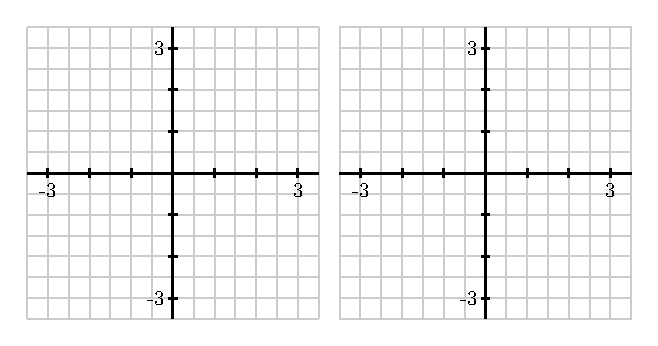
\includegraphics{figures/1_2_Ez3.eps} %\ \  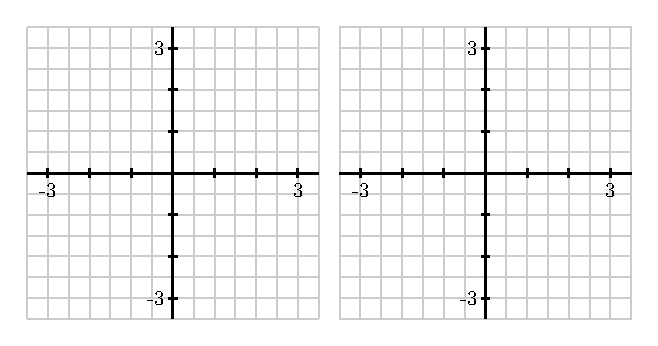
\includegraphics{figures/1_2_Ez3.eps}
   \end{center}
   \caption{Axes for plotting $y = f(x)$ in (a) and $y = g(x)$ in (b).} \label{F:1.2.Ez3}
\end{figure}
  \ea

\item A bungee jumper dives from a tower at time $t=0$. Her height  $s$ in feet at time $t$ in seconds is given by $s(t) = 100\cos(0.75t) \cdot e^{-0.2t}+100$.
	\ba
		\item Write an expression for the average velocity of the bungee jumper on the interval \\ $[1,1+h]$.
		\item Use computing technology to estimate the value of the limit as $h \to 0$ of the quantity you found in (a).
		\item What is the meaning of the value of the limit in (b)?  What are its units?
	\ea

\end{exercises}
\afterexercises